
\section{Setting up edge environments}
Unikernels, similar to traditional OSes can be booted directly from BIOS to hardware. Nevertheless, this is not flexible enough for cloud computing standarts, so hypervisors are used for on demand provisioning of unikernels. For proof of concept development, many different edge device configurations were used. There are two different usage scenarios in mind when configuring devices. First one is hypervisor enabled unikernel runtime and the other one is with IoT.

For hypervisor enabled runtime, a laptop was used. Installing a hypervisor on conventional virtual machines in cloud is a hard task because it breaks internal networking and makes it impossible to access machine from outside. Although it would be possible to make it work somehow, it's not a good testing environment as accessing to BIOS of a cloud provided virtual machine is not possible on LRZ.

This additional laptop has Debian as the host operating system and Xen was installed through Debian with administrative priviledges to access BIOS. After Xen is installed, when laptop is booted up, user can select to start debian with with Xen enabled. It's the same interface that a user sees when dual boots e.g. Windows or Linux. Starting with Xen gives access to Xen command line tool, \textbf{xl}, to manipulate dom0. Because a linux system is installed on the computer that communicates with the hypervisor, it's a straightforward process to write Kubernetes clients. That laptop is connected to Kubernetes cluster through kubeconfig.yaml and it's public IP. Figure \ref{fig:hypervisor} shows the final overview of the setup. The custom deployer is virtual-kubelet and the hypervisor square is the Xen installed laptop. Two additional linux VM's are traditional Kubernetes nodes connected with kubelet.

For testing possible deployment configurations, a linux machine with docker installed was used. While docker daemon is installed, kubelet is not installed and management of docker containers is done by virtual-kubelet. This functionality looks very similar to actual kubelet, thus it's a good exercise.

For IoT devices, Raspberry Pi 3 was used. Raspberry Pi uses ARM processor and x64 hypervisors can't be ported easily. There is also not too much motivation for it, because Raspberry Pi is not a powerful end-device and virtualisation is a resource hungry process. Nevertheless, there are projects for lightweight virtualisation on Raspberry Pi. For more powerful end devices though, there are hypervisor projects but they are out of scope for this thesis.

To experiment more with unikernel ecosystem, solo5 was also installed to the aforementioned laptop. Solo5 can be built on top of quemu or KVM and it markets itself as a unikernel specific runtime. To test solo5, Qemu was installed because the hardware didn't allow KVM virtualisation.

Another enviroment is virtual kubelet installed docker containers. Docker containers are built on top Ubuntu base image and unikernels can run on them. They are being used to simulate hundreds of IoT machines, since both docker and Raspberry Pis lack hypervisor technology.

When configuring edge devices for supervisors, a network interface for virtualisation unikernels should be set. If a unikernel application is using networking, the network interface should be given to the boot up command to make the local DHCP give it an IP.


\begin{figure}[htpb]
  
    \centering
    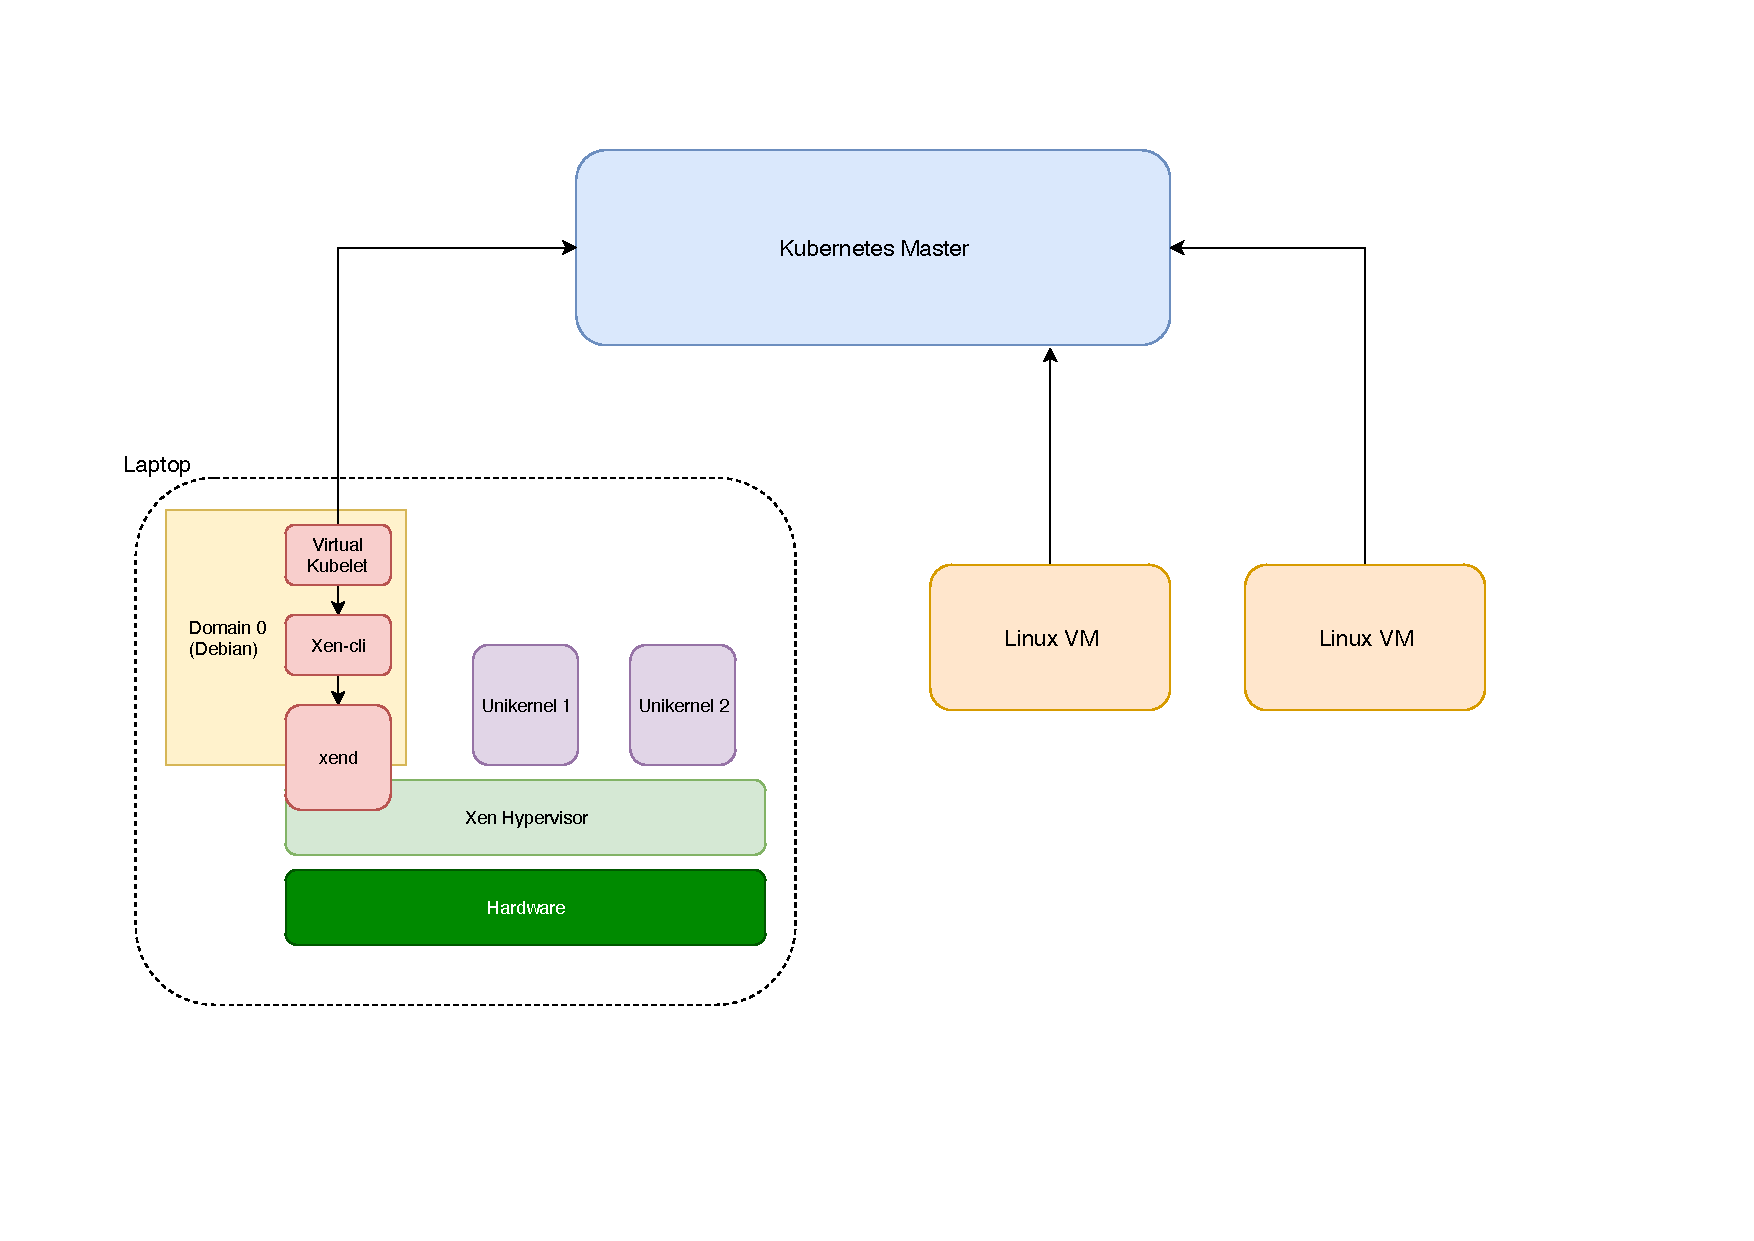
\includegraphics[width=1.2\textwidth]{figures/arch_new.pdf}
    \caption{ Kubernetes cluster with a only hypervisor enabled node for unikernel deployment} \label{fig:hypervisor}
  \end{figure}
%todo: kubeproxy
% todo: minios
